\documentclass[a4paper,oneside,14pt]{extreport}

\usepackage[T2A]{fontenc}
\usepackage[utf8]{inputenc}
\usepackage[english,russian]{babel}

\usepackage[left=30mm, right=10mm, top=20mm, bottom=20mm, bindingoffset=0cm]{geometry}

\usepackage{microtype}
\usepackage{tikz}

\usepackage{setspace}
\onehalfspacing
\usepackage{graphicx}
\usepackage{indentfirst}
\setlength{\parindent}{12.5mm}

\usepackage{titlesec}
\titleformat{\chapter}{\LARGE\bfseries}{\thechapter}{10pt}{\LARGE\bfseries}
\titlespacing*{\chapter}{0pt}{-20pt}{10pt}
\titleformat{\section}{\large\bfseries}{\thesection}{10pt}{\large\bfseries}
\titlespacing*{\section}{0pt}{0pt}{10pt}
\titleformat{\subsection}{\normalsize\bfseries}{\thesubsection}{10pt}{\normalsize\bfseries}
\titlespacing*{\subsection}{0pt}{5pt}{5pt}

\addto{\caption}{\renewcommand*{\contentsname}{Содержание}}
\usepackage[square,sort,comma,numbers]{natbib}
\renewcommand{\bibsection}{\chapter*{Список литературы}}

\usepackage{caption}

\usepackage{wrapfig}
\usepackage{float}
\usepackage{listings}
\usepackage{graphicx}
\graphicspath{{.}}
\newcommand{\imgwc}[4]
{
	\begin{figure}[#1]
		\center{\includegraphics[width=#2]{inc/img/#3}}
		\caption{#4}
		\label{img:#3}
	\end{figure}
}
\newcommand{\imghc}[4]
{
	\begin{figure}[#1]
		\center{\includegraphics[height=#2]{inc/img/#3}}
		\caption{#4}
		\label{img:#3}
	\end{figure}
}
\newcommand{\imgsc}[4]
{
	\begin{figure}[#1]
		\center{\includegraphics[scale=#2]{inc/img/#3}}
		\caption{#4}
		\label{img:#3}
	\end{figure}
}

\usepackage{pgfplots}
\pgfplotsset{compat=newest}

\usepackage{listings}
\usepackage{listingsutf8}
\lstset{
	basicstyle=\footnotesize\ttfamily,
	keywordstyle=\color{blue},
	stringstyle=\color{red},
	commentstyle=\color{gray},
	numbers=left,
	numberstyle=\tiny,
	numbersep=5pt,
	frame=false,
	breaklines=true,
	breakatwhitespace=true,
	inputencoding=utf8/koi8-r
}

\newcommand{\code}[1]{\texttt{#1}}

\usepackage{amsmath}
\usepackage{mathtools}
\usepackage{amssymb}

\usepackage[unicode]{hyperref}
\hypersetup{hidelinks}

\makeatletter
\newcommand{\vhrulefill}[1]
{
	\leavevmode\leaders\hrule\@height#1\hfill \kern\z@
}
\makeatother


\begin{document}
	\pagenumbering{Alph}
\documentclass[../report.tex]{subfiles}
\graphicspath{{\subfix{../images/}}}

\begin{document}
\thispagestyle{empty}
\doublespacing
\noindent
\begin{minipage}[l]{0.15\textwidth}
	\centering
	
\includegraphics{bmstu_low}
\end{minipage}
% нельзя делать пустую строку
\begin{minipage}[r]{0.85\textwidth}
	\centering\bfseries\singlespacing
	Министерство науки и высшего образования Российской Федерации\\
Федеральное государственное бюджетное образовательное учреждение\\
высшего образования\\
«Московский государственный технический университет\\
имени Н.Э. Баумана\\
(национальный исследовательский университет)»\\
(МГТУ им. Н.Э. Баумана)
\end{minipage}

\vspace*{5mm}
\noindent
\rule{\textwidth}{3pt}

\noindent
\MakeUppercase{Факультет}
\underline{«Информатика и системы управления»}

\noindent
\MakeUppercase{Кафедра}
\underline{«Программное обеспечение ЭВМ и информационные технологии»}

\vspace*{4cm}

\noindent
\center{
\textbf{
\MakeUppercase{Отчет\\
о лабораторной работе №5
}\\
\MakeUppercase{Конвеерная обработка данных}\\
по дисциплине:\\
«Анализ алгоритмов»
}}

\vspace*{3cm}

\begin{FlushLeft}
Руководитель: ст. преп. каф. ИУ7 \noindent\underline{\makebox[3em][l]{}} Волкова Л.Л.\\
Исполнитель: студ. гр. ИУ7-55Б \noindent\underline{\makebox[3em][l]{}} Муравьев И.А.
\end{FlushLeft}

\vspace*{\fill}
\center{
Москва 2021
}


\end{document}
\pagenumbering{arabic}
\newpage
\tableofcontents
\lstset{
	language = python,
	basicstyle=\small\sffamily,
	numbers=left,
	numberstyle=\tiny,
	stepnumber=1,
	numbersep=5pt,
	xleftmargin =.19in,
	showspaces=false,
	showstringspaces=false,
	showtabs=false,
	frame=single,
	tabsize=2,
	captionpos=t,
	breaklines=true,
	breakatwhitespace=false,
	escapeinside={\#*}{*)}
}

\newpage

\addcontentsline{toc}{chapter}{Введение}
\chapter*{Введение}
\textbf{Цель:} сравнить производительность последовательной и многопоточной версий алгоритма вычисления определителя матрицы.

\textbf{Задачи:}
\begin{enumerate}
	\item Изучить алгоритм вычисления определителя квадратной матрицы.
	\item Реализовать и протестировать:
	\begin{enumerate}
		\item последовательный алгоритм нахождения определителя матрицы;
		\item многопоточный алгоритм нахождения определителя матрицы.
	\end{enumerate}
	\item Провести сравнительный анализ алгоритмов по затрачиваемым ресурсам (процессорному времени работы).
	\item Определить, всегда ли при задании количества потоков, равному удвоенному количеству логических ядер процессора, достигается наибольшая эффективность.
\end{enumerate}
\newpage

\chapter{Аналитическая часть}
 Многопоточность — способность центрального процессора (CPU) или одного ядра
в многоядерном процессоре одновременновыполнять несколько процессов или
потоков, соответствующим образом поддерживаемых операционной системой.

Этот подход отличается от многопроцессорности, так как многопоточность
процессов и потоков совместно использует ресурсы одного или нескольких ядер:
вычислительных блоков, кэш-памяти ЦПУ или буфера перевода с преобразованием (TLB).

В тех случаях, когда многопроцессорные системы включают в себя несколько полных блоков обработки,
многопоточность направлена на максимизацию использования ресурсов одного ядра,
используя параллелизм на уровне потоков или на уровне инструкций.

Поскольку эти два метода являются взаимодополняющими,
их иногда объединяют в системах с несколькими многопоточными ЦП
и в ЦП с несколькими многопоточными ядрами.
Смысл многопоточности — квазимногозадачность на уровне одного исполняемого процесса.

Многопоточность (как доктрину программирования) не следует путать ни с многозадачностью,
ни с многопроцессорностью, несмотря на то, что операционные системы,
реализующие многозадачность, как правило, реализуют и многопоточность.

Достоинства:
\begin{itemize}
	\item облегчение программы посредством использования общего адресного пространства;
	\item меньшие затраты на создание потока в сравнении с процессами;
	\item повышение производительности процесса за счёт распараллеливания процессорных вычислений;
	\item если поток часто теряет кэш, другие потоки могут продолжать
	использовать неиспользованные вычислительные ресурсы.
\end{itemize}

Недостатки:
\begin{itemize}
	\item несколько потоков могут вмешиваться друг в друга при совместном
	использовании аппаратных ресурсов \cite{Nemirovsky};
	\item с программной точки зрения аппаратная поддержка многопоточности
	более трудоемка для программного обеспечения \cite{Olukotun};
	\item проблема планирования потоков;
	\item специфика использования. Вручную настроенные программы на ассемблере,
	использующие расширения MMX или AltiVec и выполняющие предварительные выборки данных,
	не страдают от потерь кэша или неиспользуемых вычислительных ресурсов.
	Таким образом, такие программы не выигрывают от аппаратной многопоточности
	и действительно могут видеть ухудшенную производительность из-за конкуренции за общие ресурсы.
\end{itemize}
	Однако несмотря на количество недостатков, перечисленных выше,
	многопоточная парадигма имеет большой потенциал на сегодняшний день,
	и при должном написании кода позволяет значительно ускорить однопоточные алгоритмы.
	
	Определитель матрицы или просто определитель играет важную роль в решении систем линейных уравнений.
	Определитель матрицы $A$ обозначается как $\det A$, $\Delta A$, $|A|$
	
	Сформулировать определение определителя матрицы можно на основе его свойств.
	Определителем вещественной матрицы называется функция $\det{}: \mathbb{R}^{n\times n} \rightarrow \mathbb{R}$,
	обладающая следующими свойствами:
	
	\begin{enumerate}
		\item $\det{(A)}$ - кососимметрическая функция строк (столбцов) матрицы $A$
		\item $\det{(A)}$ - полилинейная функция строк(столбцов) матрицы $A$
		\item $\det{(A)} = 1$, где $E$ - единичная $n \times n$-матрица
	\end{enumerate}
	
\section{Нахождение определителя матрицы}
Ниже описаны способы нахождения определителя матрицы размеров $1 \times 1$, $2 \times 2$, $3 \times 23$, $n \times 1n$.

\subsection{Матрица $1 \times 1$}
Для матрицы первого порядка значение детерминанта равно единственному элементу этой матрицы:

\begin{equation}
\label{eq:det_1x1}
\delta  = |a_{11}| = a_{11}
\end{equation}

\subsection{Матрица $2 \times 2$}
Для матрицы $2 \times 2$ определитель вычисляется следующим образом:

\begin{equation}
\label{eq:det_2x2}
\Delta = \begin{vmatrix}
a & c \\
b & d
\end{vmatrix} = ad - bc
\end{equation}
Абсолютное значение определителя $|ad - bc|$ равно площади параллелограмма с вершинами
$(0, 0), (a, b), (a + c, b + d), (c, d)$.

\subsection{Матрица $3 \times 3$}
Определитель матрицы $3 \times 3$ можно вычислить по формуле:
\begin{equation}
\label{eq:det_3x3}
\begin{aligned}
\Delta = \begin{vmatrix}
a_{11} & a_{12} & a_{13} \\
a_{21} & a_{22} & a_{23} \\
a_{31} & a_{32} & a_{33}
\end{vmatrix} =
a_{11} \cdot \begin{vmatrix}
a_{22} & a_{23} \\
a_{32} & a_{33}
\end{vmatrix}
-
a_{12} \cdot \begin{vmatrix}
a_{21} & a_{23} \\
a_{31} & a_{33}
\end{vmatrix}
+
a_{13} \cdot \begin{vmatrix}
a_{21} & a_{22} \\
a_{31} & a_{32}
\end{vmatrix}
=
a_{11}a_{22}a_{33} - a_{11}a_{23}a_{32} - a_{12}a_{21}a_{33} +
a_{12}a_{23}a_{31} + a_{13}a_{21}a_{32} - a_{13}a_{22}a_{31}
\end{aligned}
\end{equation}

Определитель матрицы, составленной из векторов $a, b, c$ представляет
собой объём параллелепипеда, натянутого на вектора $a, b, c$.

\subsection{Матрица $n \times n$}
В общем случае, для матриц $n \times n$, где $n > 2$ определитель можно вычислить,
применив следующую рекурсивную формулу:

\begin{equation}
\label{eq:det_nxn}
\Delta =
\sum\limits_{j = 1}^{n} (-1)^{1 + j} \cdot a_{1j} \cdot M_{j}^{-1}
, \text{ где} M_{j}^{-1} - дополнительный минор к элементу a_{ij}
\end{equation}

В данной лабораторной работе стоит задача распараллеливания алгоритма нахождения определителя матрицы.
Так как каждое слагаемое для вычисления итогового определителя
вычисляется независимо от других и матрица не изменяется, для параллельного вычисления определителя
было решено распределять задачу вычисления слагаемых между потоками.

\section{Вывод}
Был рассмотрен алгоритм нахождения определителя квадратной матрицы размера $n \times n$, он независимо вычисляет слагаемые
для нахождения итогового определителя, что дает возможность для реализации параллельного варианта алгоритма.
\newpage

\chapter{Конструкторская часть}
Данный раздел содержит требования к разрабатываемому ПО, схемы реализуемых в работе алгоритмов (стандартного рекурсивного алгоритма вычисления определителя матриц и алгоритма с использованием потоков в виде схем потока-диспетчера и рабочего потока) и теоретический расчет повышения эффективности исполнения алгоритма по времени.

\section{Требования к программному обеспечению}
Требования, выдвигаемые к разрабатываемому ПО:
\begin{itemize}
	\item входные данные - размер матрицы (целое число), её элементы (вещественные числа);
	\item выходные данные - определитель матрицы (вещественное число).
\end{itemize}

\section{Схемы алгоритмов}
В данном пункте раздела представлены схемы реализуемых в работе алгоритмов.

На рисунке~\ref{img:count_det} представлена схема рекурсивного алгоритм нахождения определителя.
\begin{figure}[H]
	\centering
	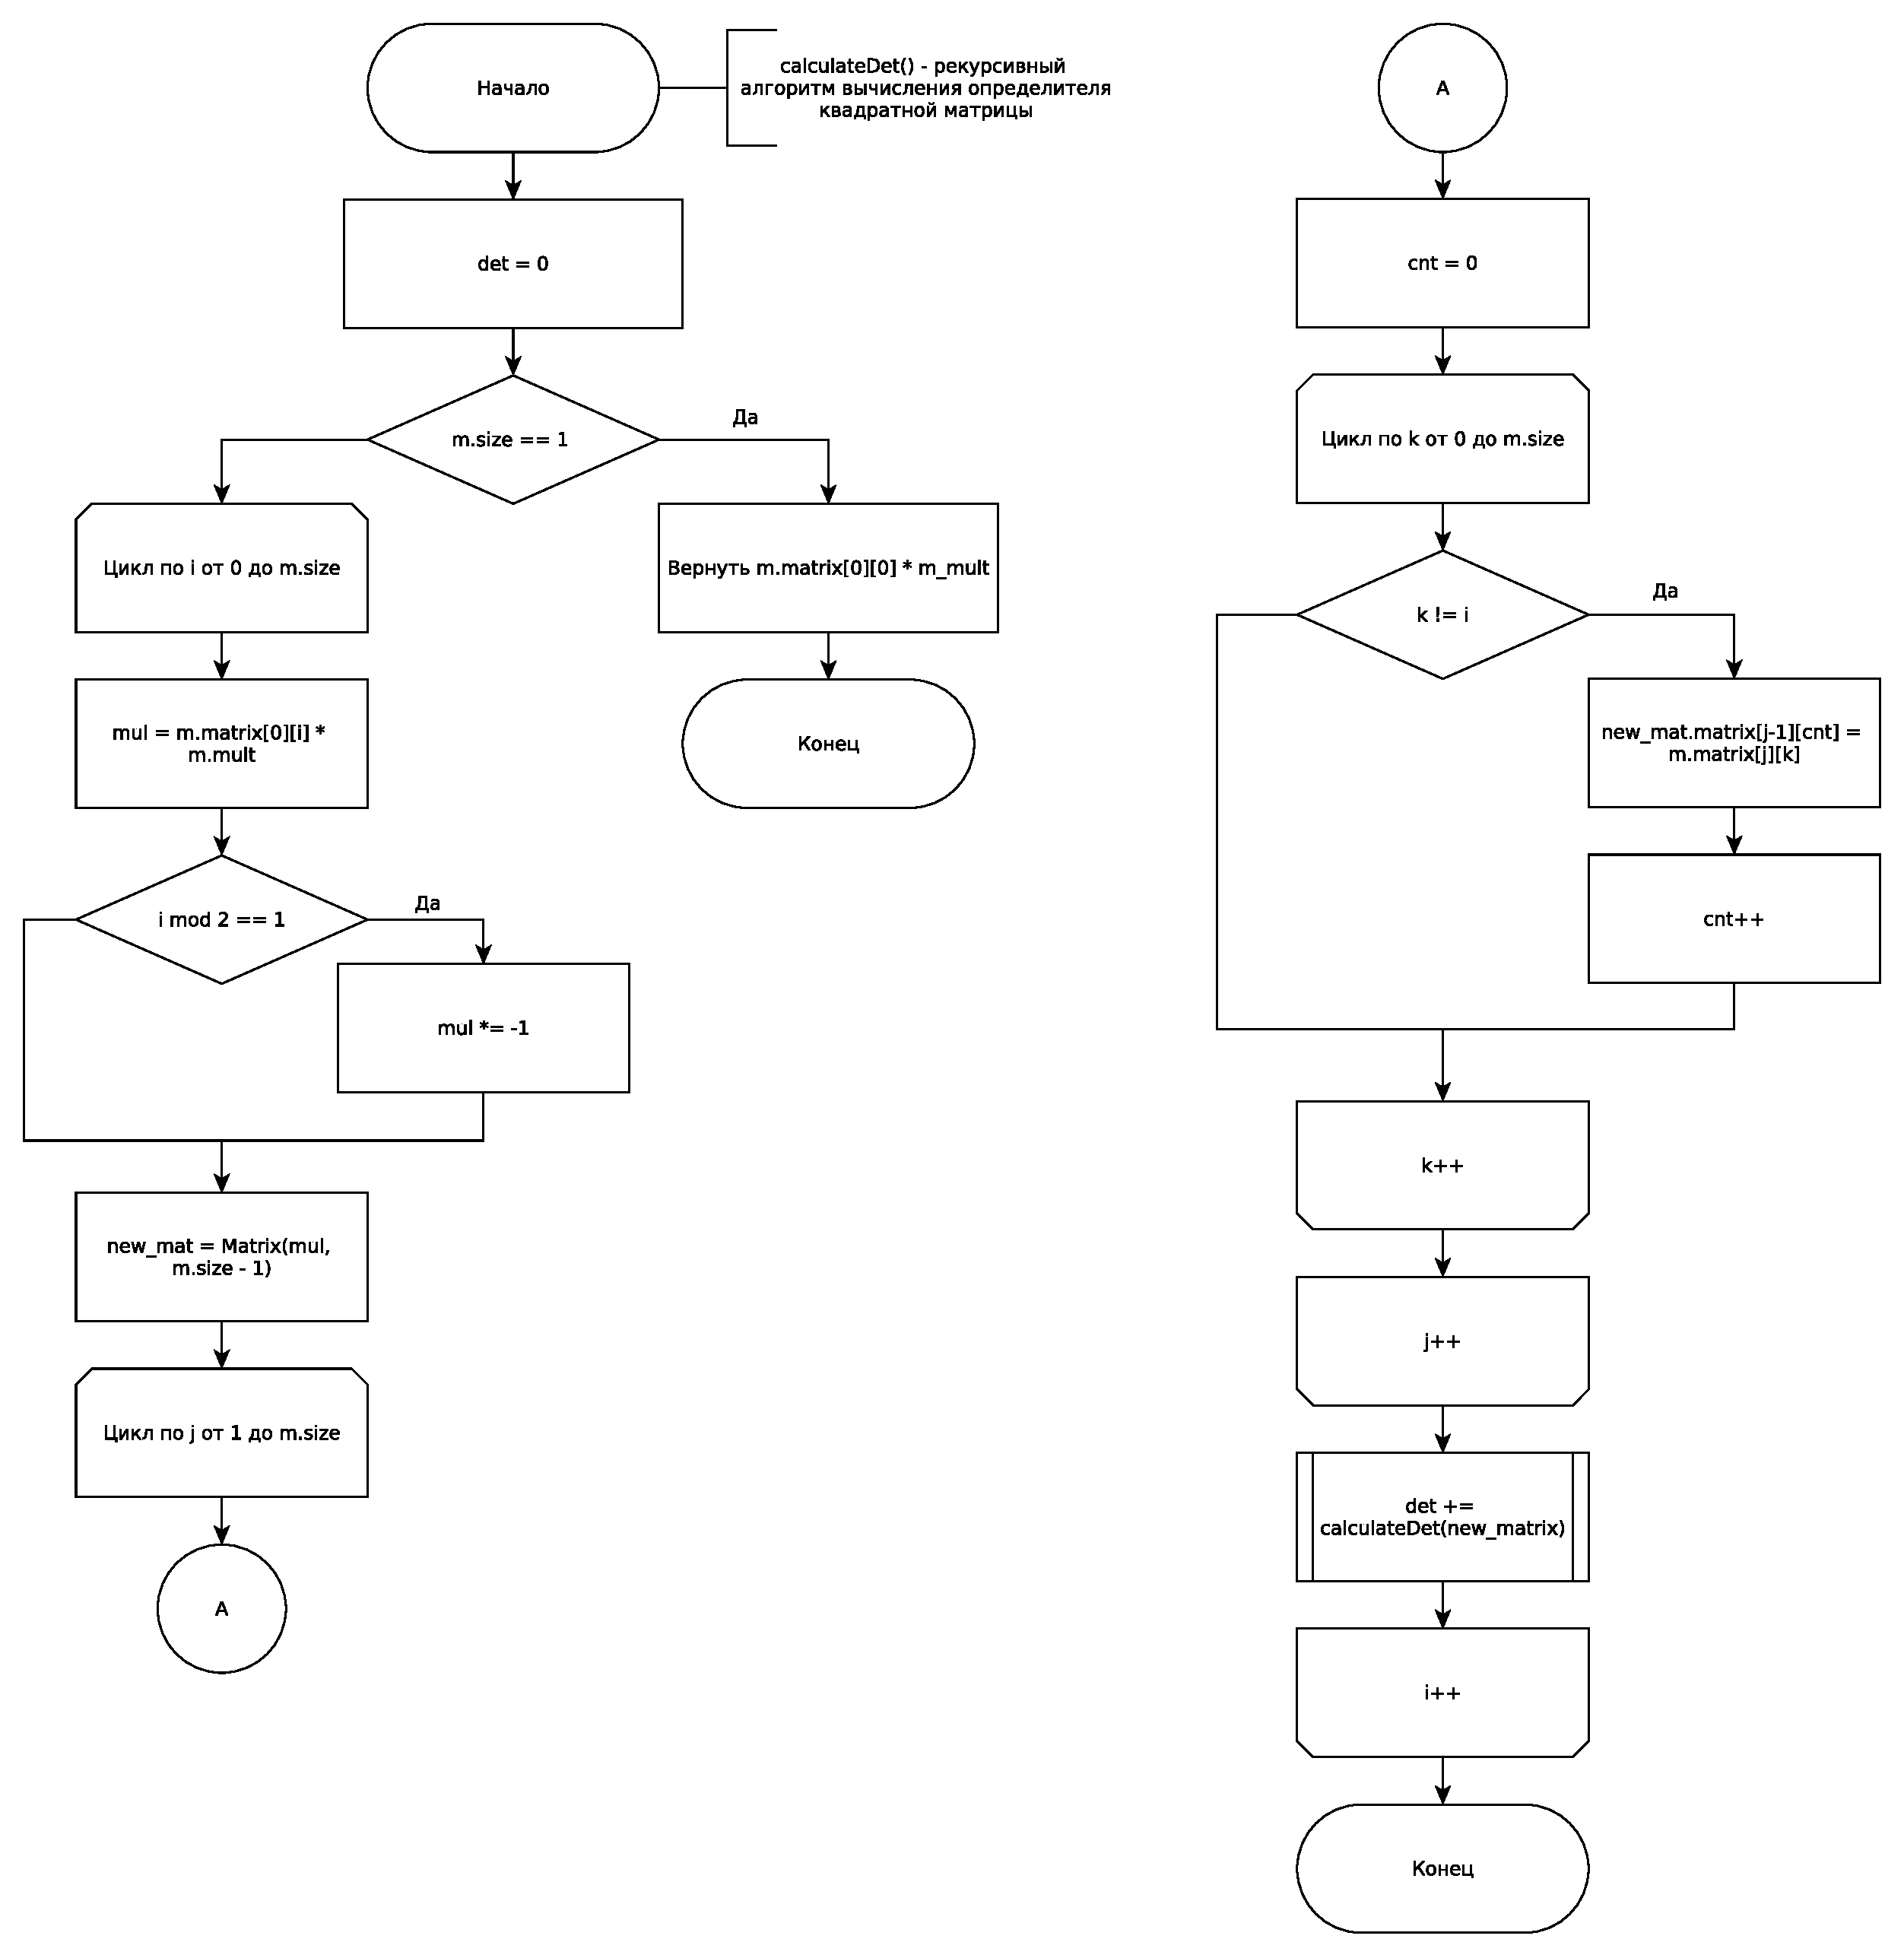
\includegraphics[width=1.00\linewidth]{images/count_det}
	\caption{Схема рекурсивного алгоритма нахождения определителя}
	\label{img:count_det}
\end{figure}

На рисунке~\ref{img:thread_schema} представлена схема алгоритма подсчета слагаемых итогового определителя матрицы
при использовании потоков.

\begin{figure}[H]
	\centering
	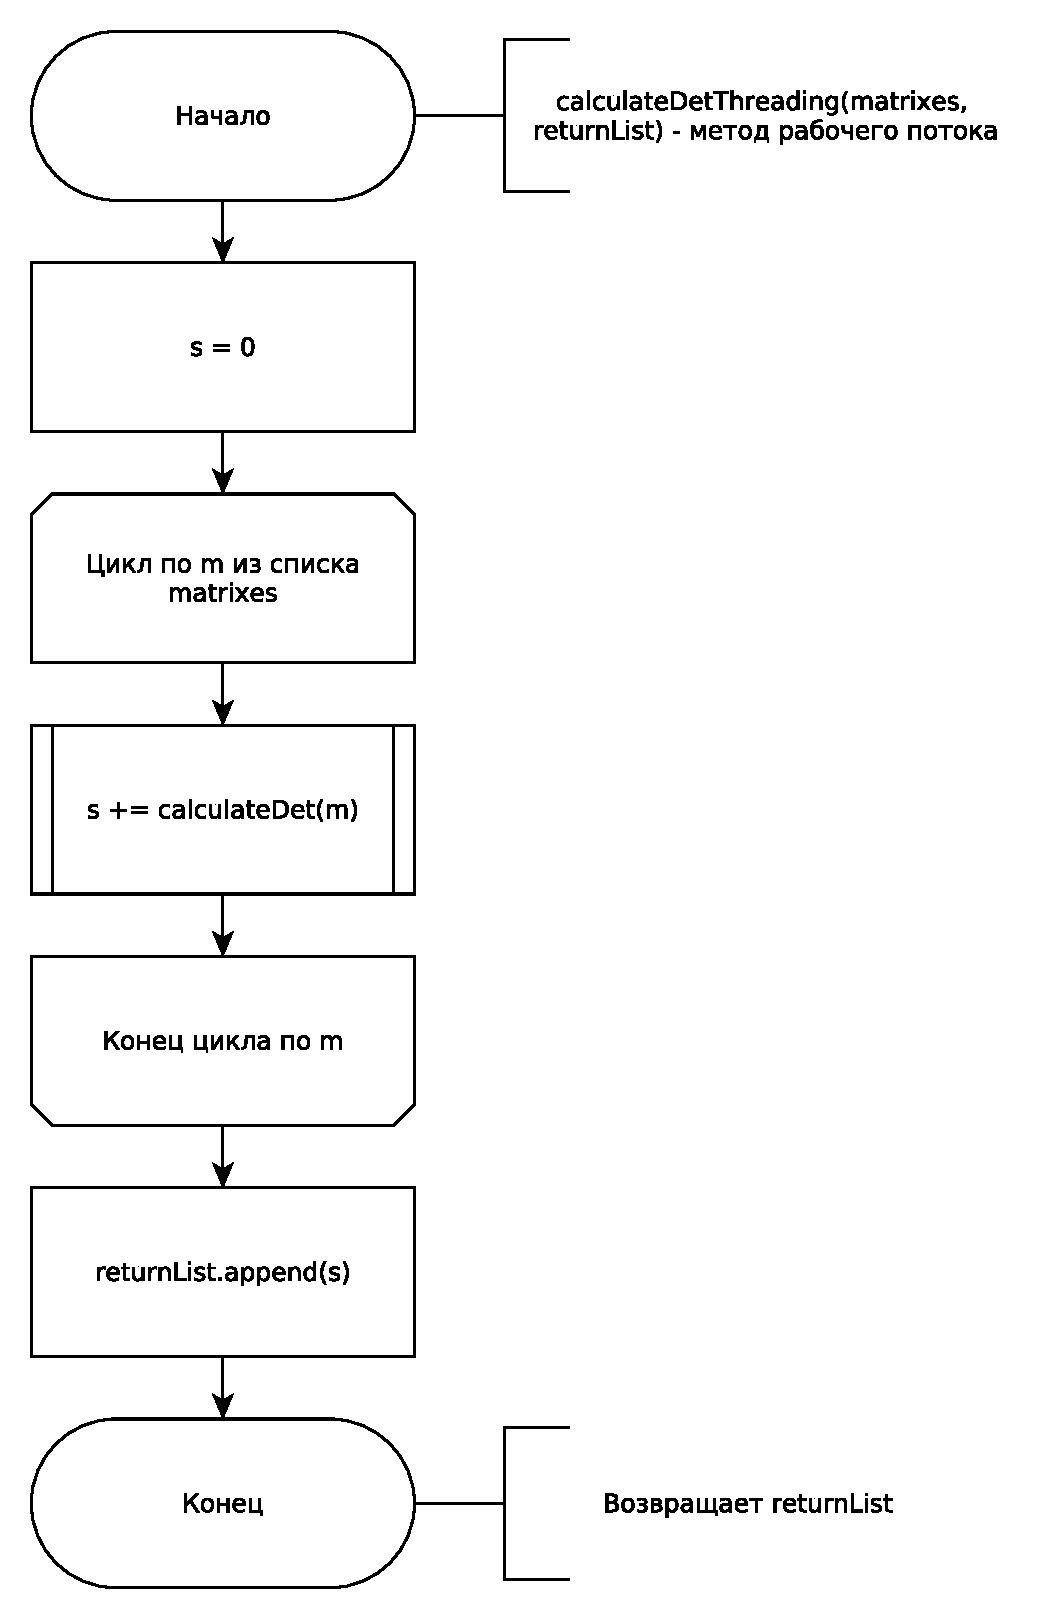
\includegraphics[width=0.85\linewidth]{images/thread_schema}
	\caption{Схема рекурсивного алгоритм нахождения определителя}
	\label{img:thread_schema}
\end{figure}

На рисунках~\ref{img:solver_1} -~\ref{img:solver_2} представлена схема алгоритма создания потоков,
разделения задач между ними и нахождения итогового определителя матрицы.

\begin{figure}[H]
	\centering
	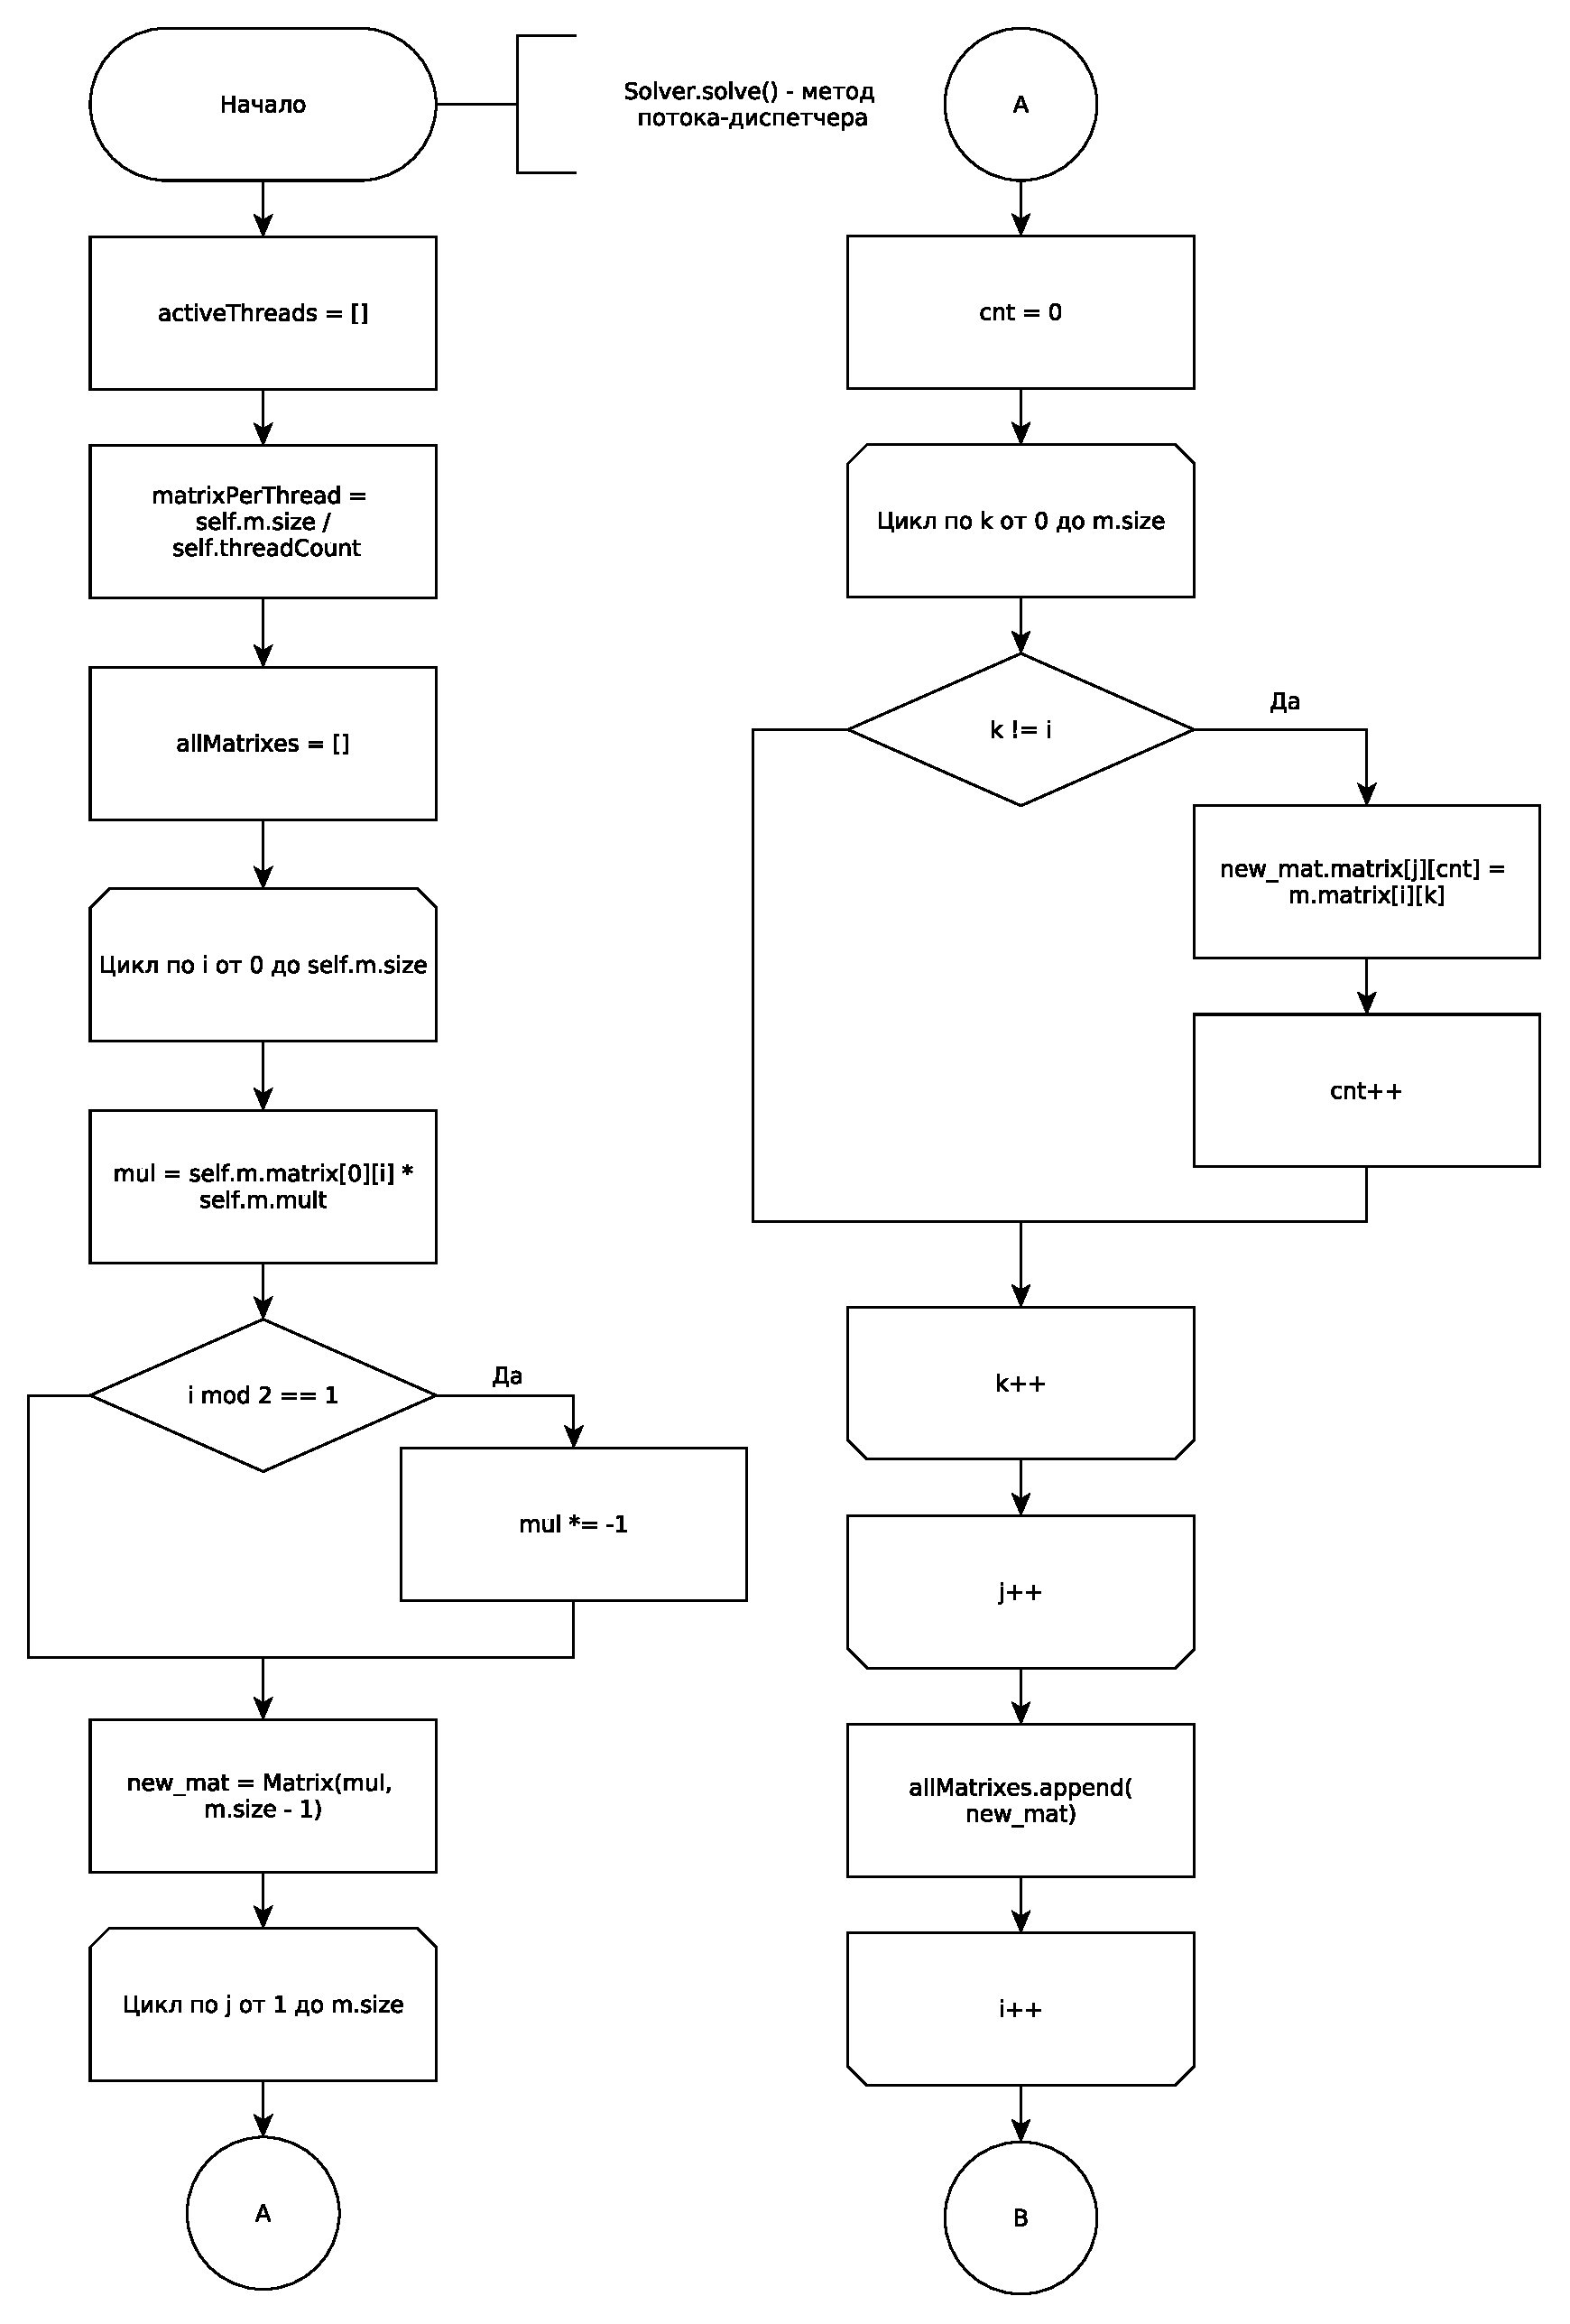
\includegraphics[width=0.85\linewidth]{images/solver_part_1}
	\caption{Схема рекурсивного алгоритм нахождения определителя}
	\label{img:solver_1}
\end{figure}

\begin{figure}[H]
	\centering
	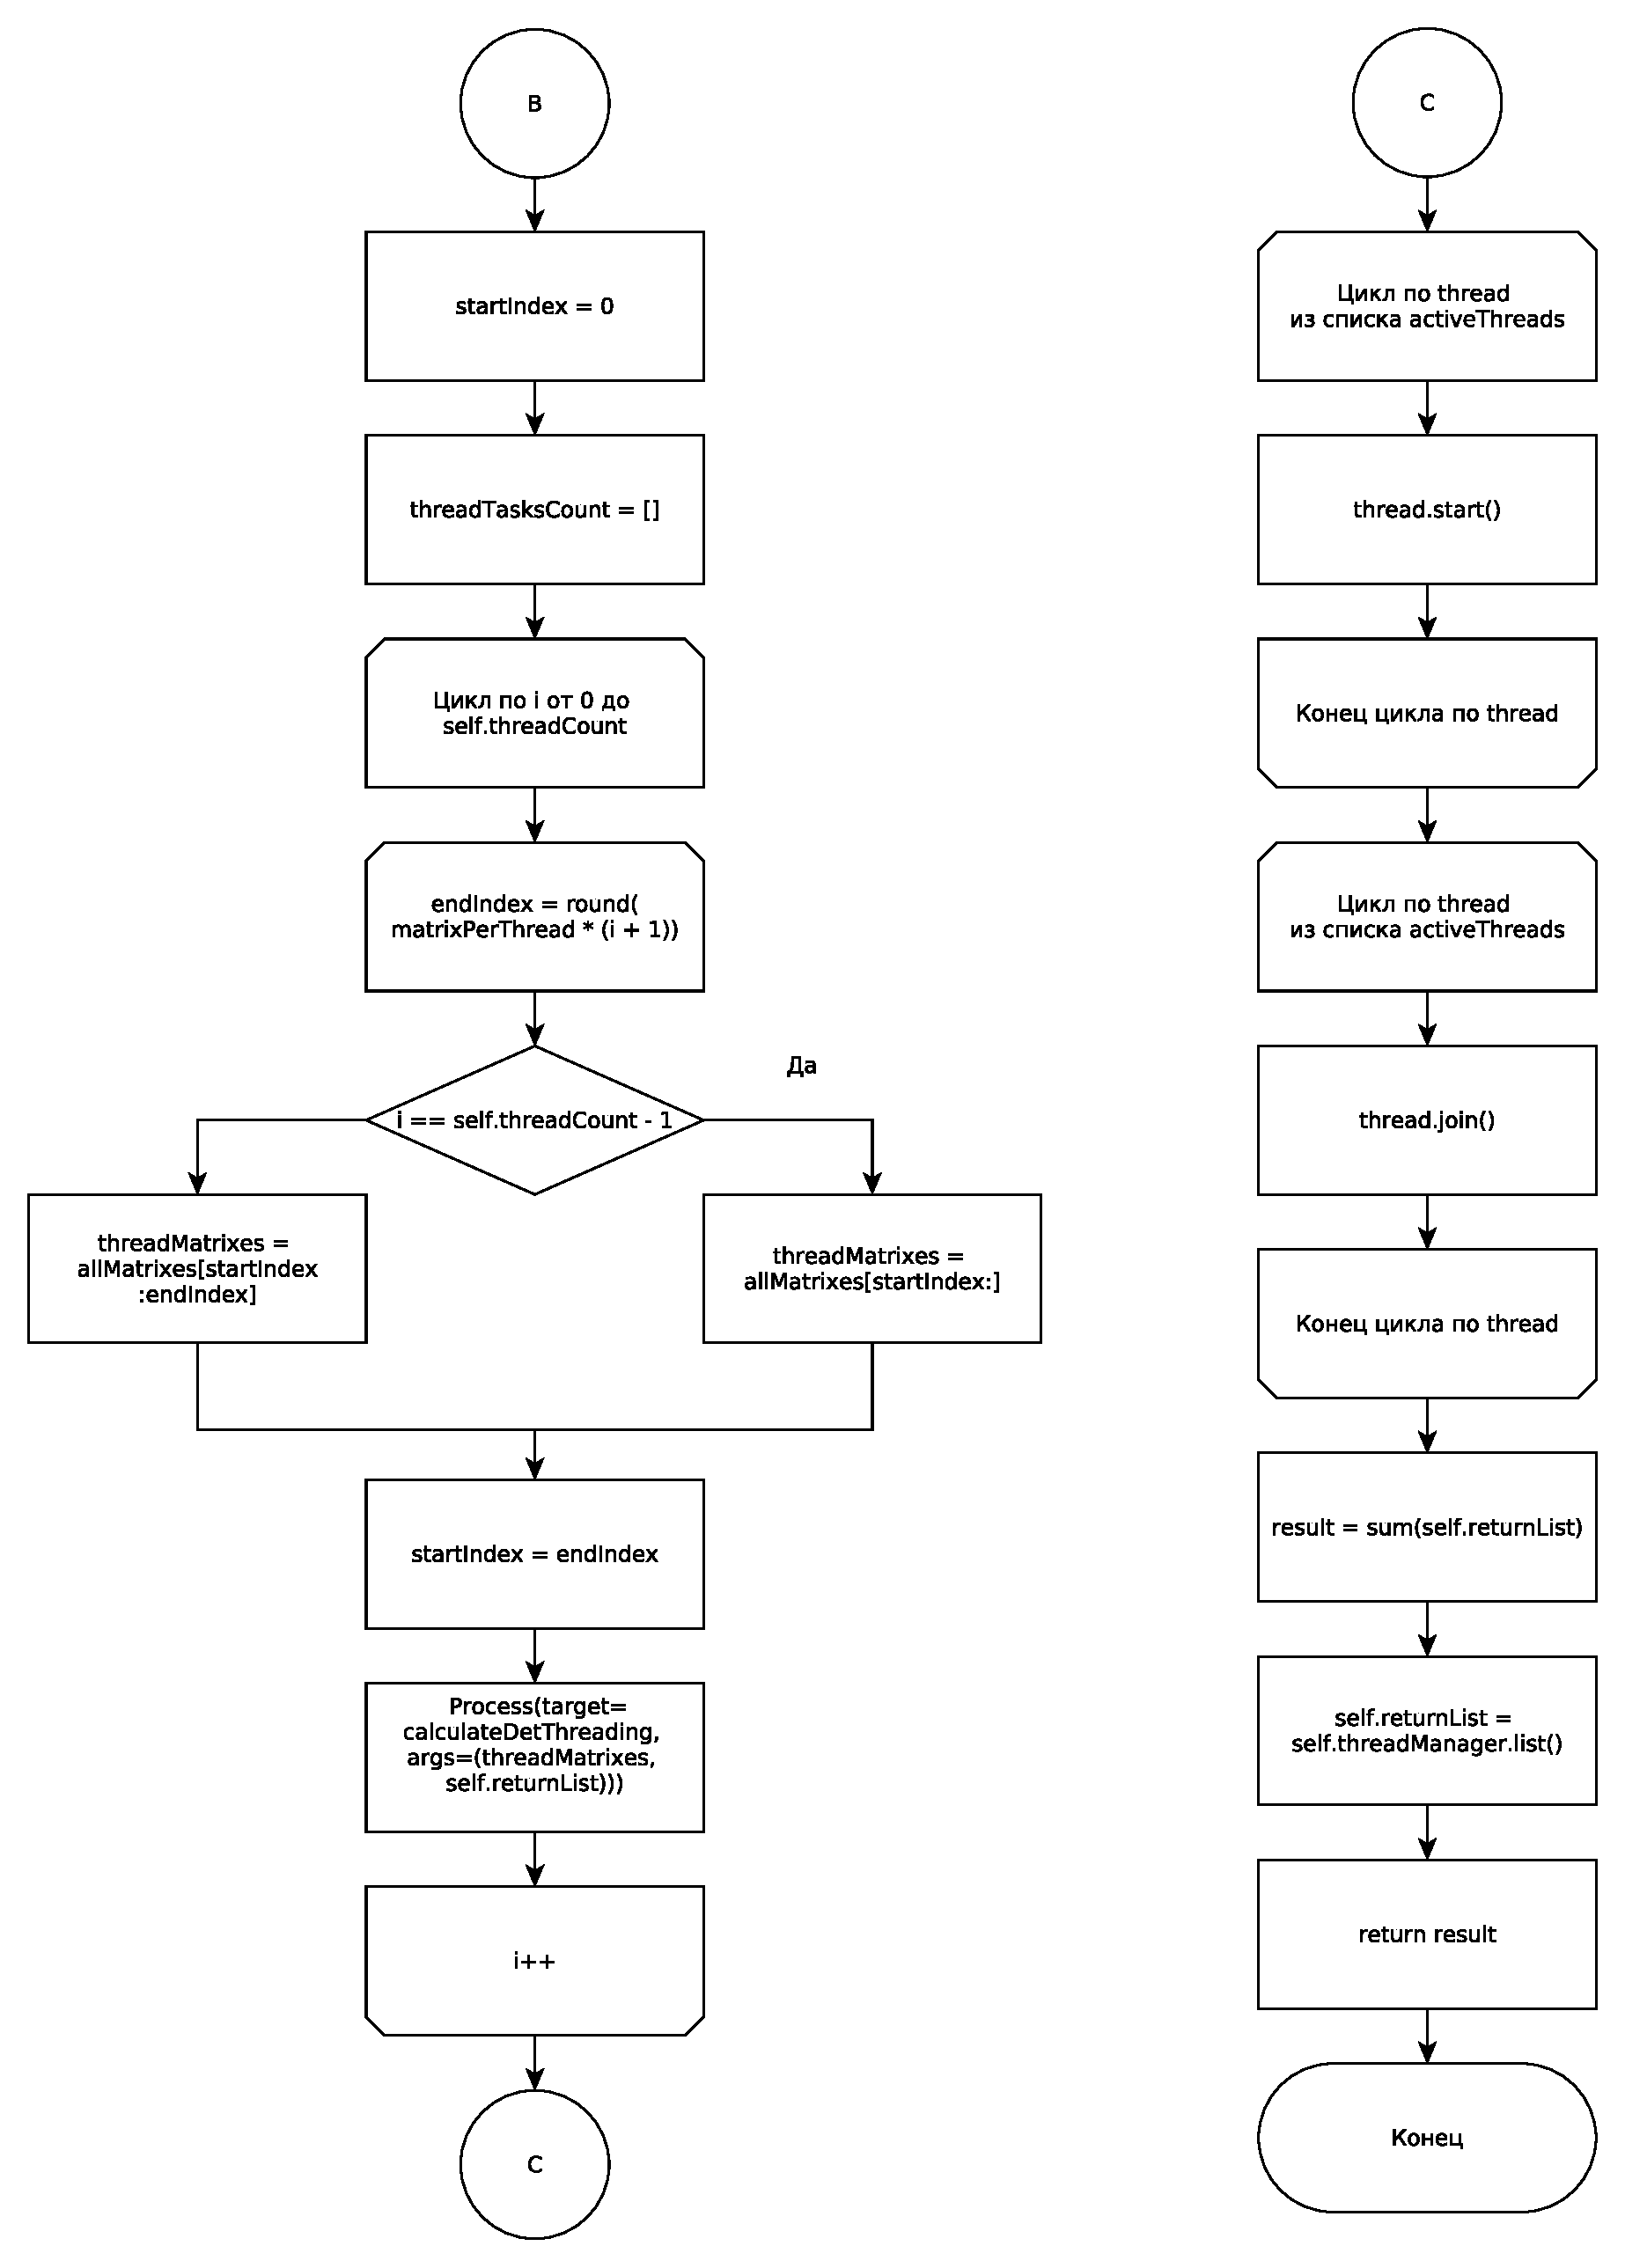
\includegraphics[width=0.90\linewidth]{images/solver_part_2}
	\caption{Схема рекурсивного алгоритм нахождения определителя}
	\label{img:solver_2}
\end{figure}

\section{Вывод}
В данном разделе на основе приведенных в аналитическом разделе теоретических данных были составлены схемы алгоритмов для реализации в технологической части, в том числе, разделение вычисления определителя на потоки. 

\chapter{Технологическая часть}
Данный раздел содержит обоснование выбора языка и среды разработки, реализацию алгоритмов.

\section{Средства реализации}
Для реализации программы был выбран язык программирования Python~\cite{python}. Такой выбор обусловлен следующими причинами:
\begin{itemize}
	\item имеется большой опыт разработки;
	\item имеет большое количество расширений и библиотек, в том числе библиотеку для работы с потоками, измерения времени, построения графиков;
	\item обладает информативной документацией;
\end{itemize}

\section{Реализация алгоритмов}
В листингах \ref{lst:det_rec} - \ref{lst:work_thread} представлены реализации рассматриваемых алгоритмов.
%\newpage
\captionsetup{singlelinecheck=false, justification=raggedright}
\begin{lstlisting}[caption=Рекурсивный алгоритм вычисления определителя матрицы, label={lst:det_rec}]
def calculateDet(m: Matrix):
	s = 0                                                   
	if m.size == 1:                                         
		s = m.matrix[0][0] * m.mult                         
	else:                                                   
		for i in range(m.size):                             
			mul = m.matrix[0][i] * m.mult
			if i % 2 == 1:               
				mul *= -1                    
			size = m.size - 1            
			new_mat = Matrix(size, mul)  
			for j in range(1, m.size):   
				cnt = 0                      
				for k in range(m.size):      
					if k != i:                   
						new_mat.matrix[j - 1][cnt] = m.matrix[j][k] 
						cnt += 1                                    
			s += calculateDet(new_mat)                  
	return s      
\end{lstlisting}

\begin{lstlisting}[caption=Поток-диспетчер (часть 1)]
class Dispatcher:
	def __init__(self, size: int = 0, matrix: Matrix = None):
		self.m = matrix
		if size == 0: 
			size = 9
		if self.m is None:
			self.m = Matrix(size).randomize()
		self.threadCount = 1
		self.threadManager = Manager()
		self.returnList = self.threadManager.list()
	
	def dispatch(self):
		activeThreads = []
		matrixPerThread = self.m.size / self.threadCount
		allMatrixes = []
		for i in range(self.m.size):
			mul = self.m.matrix[0][i] * self.m.mult
			if i % 2 == 1:
				mul *= -1
			size = self.m.size - 1
			matrix = []
			for j in range(1, self.m.size):
				matrix.append([])
				for k in range(self.m.size):
					if k != i:
						matrix[-1].append(self.m.matrix[j][k])
			allMatrixes.append(Matrix(size, mul, matrix))
		startIndex = 0
		threadTasksCount = []
		for i in range(self.threadCount):
			endIndex = round(matrixPerThread * (i + 1))
			if i == self.threadCount - 1:  # last thread
				threadMatrixes = allMatrixes[startIndex:]
			else:
				threadMatrixes = allMatrixes[startIndex:endIndex]
			startIndex = endIndex
			activeThreads.append(
			Process(target=calculateDetThreading, args=(threadMatrixes, self.returnList)))
			threadTasksCount.append(len(threadMatrixes))
\end{lstlisting}
\begin{lstlisting}[caption=Поток-диспетчер (часть 2)]
		for thread in activeThreads:
			thread.start()
		for thread in activeThreads:
			thread.join()
		result = sum(self.returnList)
		self.returnList = self.threadManager.list()
		return result
\end{lstlisting}
%\newpage
\begin{lstlisting}[caption=Рабочий поток, label={lst:work_thread}]
def calculateDetThreading(matrixes, returnList: list):
	s = 0
	for m in matrixes:
		s += calculateDet(m)
	returnList.append(s)
\end{lstlisting}

\section{Тестирование}
В таблице \ref{tab:tests} представлены использованные для тестирования методом "черного ящика" данные, были рассмотрены все возможные тестовые случаи. Все тесты пройдены успешно.

\begin{table}[H]
	\begin{center}
		\captionsetup{justification=raggedleft, singlelinecheck=false}
		\caption[]{\label{tab:tests} Проведенные тесты}

	\begin{tabular}{|c|c|}
		\hline
		\rule[-1ex]{0pt}{2.5ex} Матрица & Определитель \\
		\hline
		\rule[-1ex]{0pt}{2.5ex} $\begin{pmatrix}
		9
		\end{pmatrix}$ & 9
		\\
		\hline
		\rule[-1ex]{0pt}{2.5ex} $\begin{pmatrix}
			0 & 0 \\
			0 & 0
		\end{pmatrix}$ & 0
		\\
		\hline
		\rule[-1ex]{0pt}{2.5ex} $\begin{pmatrix}
			1 & 0 & 0 \\
			0 & 1 & 0 \\
			0 & 0 & 1
		\end{pmatrix}$ & 1
		 \\
		\hline
		\rule[-1ex]{0pt}{2.5ex}	$\begin{pmatrix}
			1 & 2 & 3 \\
			4 & 5 & 6 \\
			7 & 8 & 12
		\end{pmatrix}$ & -9
		\\
		\hline
		\rule[-1ex]{0pt}{2.5ex} $\begin{pmatrix}
			1 & 2 & 3 & 4 \\
			5 & 6 & 7 & 8 \\
			9 & 10 & 11 & 12 \\
			13 & 14 & 15 & 16
		\end{pmatrix}$ & 0
		 \\
		 \hline
	\end{tabular}
\end{center}
\end{table}
\section{Выводы}
В данном разделе были реализованы и протестированы алгоритмы рекурсивного вычисления определителя и вычисления определителя с использованием многопоточности.
\newpage

\chapter{Экспериментальная часть}
В данном разделе сравниваются реализованные алгоритмы, дается сравнительная оценка затрат на время.

\section{Пример работы программы}
Пример работы программы представлен на рисунках \ref{fig:input_mat_ex} - \ref{fig:gener_ex}.
\captionsetup{singlelinecheck=true}
\begin{figure}[H]
	\centering
	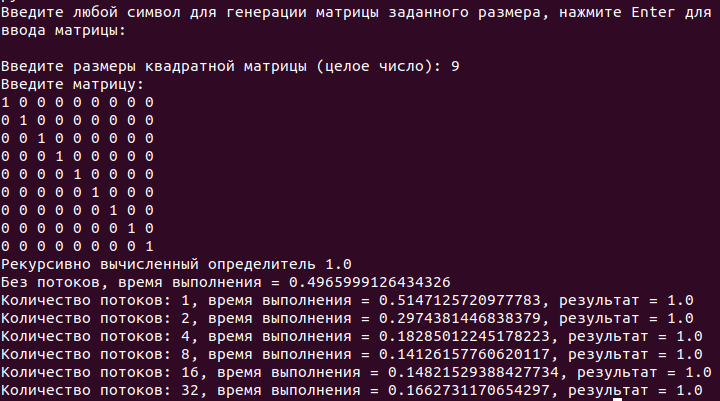
\includegraphics[width=1\linewidth]{images/input_mat_ex}
	\caption{Пример работы программы для вводимой матрицы}
	\label{fig:input_mat_ex}
\end{figure}

\begin{figure}[H]
	\centering
	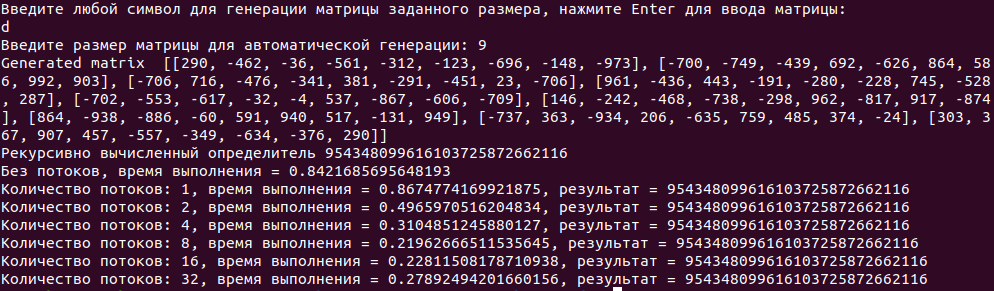
\includegraphics[width=1\linewidth]{images/generate_ex}
	\caption{Пример работы программы для вводимой матрицы}
	\label{fig:gener_ex}
\end{figure}


\section{Технические характеристики}
Технические характеристики устройства, на котором выполнялось исследование:
\begin{itemize}
	\item операционная система: Ubuntu 20.01 Linux x86\_64~\cite{ubuntu};
	\item оперативная память: 8 Гб;
	\item процессор: AMD Ryzen5 4500U~\cite{processor}:
	\begin{itemize}
		\item количество физических ядер: 6;
		\item количество логических ядер: 6.
	\end{itemize}
\end{itemize}

\section{Время выполнения алгоритмов}
Время выполнения алгоритмов измерялось на автоматически генерируемых квадратных матрицах необходимого размера (элементы которых - вещественные числа в диапазоне [-1000, 1000]) с использованием функции time библиотеки time. Усредненные результаты 10 замеров реального времени работы приведены в таблице ниже.

На рисунке \ref{fig:graph} представлена зависимость времени вычисления определителя матриц от размеров на основе таблицы \ref{tab:time}. Для матриц, размерность которых меньше 6, вычисление с использованием потоков занимает минимум в 1.3 раз (с увеличением коэффициента при увеличении количества потоков) больше времени в связи с превышением затратами на создание потоков затрат на последовательное вычисление определителя. Однако с увеличением размеров матрицы становится заметным преимущество использования параллельных вычислений. Таким образом, использование двух потоков дает выигрыш от 1.2 до 1.7 раз (для матриц, больших $6\times6$), четырех - от 1.2 до 2.8 раз (для матриц, больших $6\times6$), восьми - от 1.6 до 3.5 раз (матрицы от $7\times7$), шестнадцати - от 2.7 до 4.4 раз, для двадцати четырех - от 2.3 до 4.28 раз (матрицы от $8\times8$). Таким образом, с увеличением размерности матрицы, выигрыш от использования потоков увеличивается, при этом набольшим приростом, несмотря на получение преимуществ для матриц больших, чем те, на которых начинает выигрывать использование двух потоков ($6\times6$), обладает использование шестнадцати потоков, причем с ростом размерности матрицы выигрыш увеличивается соразмерно количеству потоков. Исключением является использование 24 потоков, который уступает в эффективности 16-и потокам из-за увеличения затрат на содержание потоков и управления ими.
\begin{table}[H]
	\begin{center}
		\captionsetup{justification=raggedleft, singlelinecheck=false}
		\caption{\label{tab:time} Время вычисления определителя матриц разных размеров в миллисекундах}
		\begin{tabular}{|c c c c c c c|} 
			\hline
			Размер&1 поток&2 потока&4 потока&8 потоков&16 потоков&24 потока\\ [0.5ex]
			\hline
	   		   4 &   12 &   14 &   16 &   22 &   36 &   51
	   		\\ 
	   		\hline
	   		5 &   14 &   15 &   16 &   23 &   37 &   51
	   		\\ 
	   		\hline
	   		6 &   22 &   18 &   19 &   23 &   37 &   50
	   		\\ 
	   		\hline
	   		7 &   50 &   33 &   29 &   31 &   46 &   58
	   		\\ 
	   		\hline
	   		8 &  251 &  138 &   80 &   83 &   94 &  108
	   		\\ 
	   		\hline
	   		9 & 2102 & 1212 &  756 &  599 &  476 &  491
	   		\\ 
	   		\hline
		\end{tabular}
	\end{center}
\end{table}

\begin{figure}[H]
	\centering
	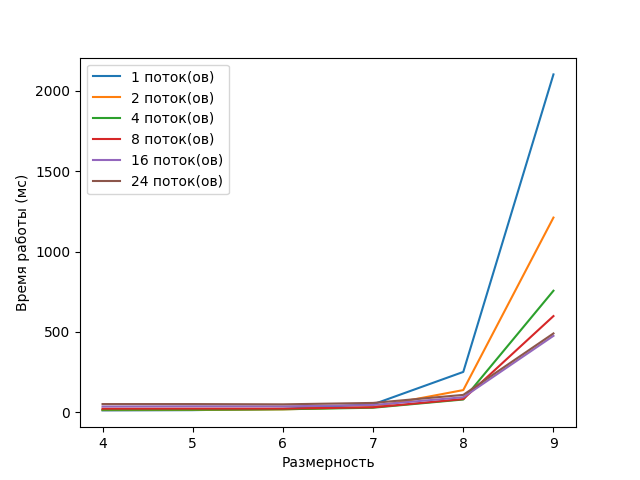
\includegraphics[width=0.9\linewidth]{images/graph}
	\caption{Зависимость времени работы алгоритмов от размера квадратной матрицы}
	\label{fig:graph}
\end{figure}

\section{Выводы}
В данном разделе были проведены измерения времени, затрачиваемого на вычисление определителя матрицы с использованием параллельных вычислений и без них.
На матрицах, размер которых не превышает 5, параллельные версии алгоритма оказались неэффективны. С увеличением размеров увеличивается эффективность использования параллельных вычислений, причем чем больше количество процессов, тем позже появляется выигрыш, но тем более существенным он оказывается. Исключением является использование 24 потоков в связи с большими затратами на обслуживание потоков в ядрах по сравнению с меньшим количеством потоков. Таким образом, выигрыш для 4 и 8 потоков проявляется на матрицах, больших $6\times6$ и составляет от 1.2 до 1.7 раз и от 1.2 до 2.8 раз соответственно, для восьми потоков - на матрицах, больших $7\times7$, от 1.5 до 3.5 раз, для 16 и 24 потоков - на матрицах, больших $8\times8$, от  2.7 до 4.4 раз и от 2.3 до 4.28 раз соответственно.
\newpage

\addcontentsline{toc}{chapter}{Заключение}
\chapter*{Заключение}
В процессе выполнения лабораторной работы были изучены и реализованы алгоритмы последовательного и параллельного вычисления определителя квадратной матрицы.

Было исследовано время выполнения выше обозначенных алгоритмов. В результате было выявлено, что на матрицах, размер которых не превышает 5, использование параллельных вычислений нецелесообразно из-за превышения затратами на содержание потоков затрат на последовательное вычисление определителя. С увеличением размеров увеличивается эффективность использования параллельных вычислений, причем чем больше количество процессов, тем позже появляется выигрыш, но тем более существенным он оказывается. Исключением является использование 24 потоков в связи с увеличением затрат на обслуживание потоков в ядрах по сравнению с 16 потоками. Таким образом, выигрыш для 4 и 8 потоков проявляется на матрицах, больших $6\times6$ и составляет от 1.2 до 1.7 раз и от 1.2 до 2.8 раз соответственно, для восьми потоков - на матрицах, больших $7\times7$, от 1.5 до 3.5 раз, для 16 и 24 потоков - на матрицах, больших $8\times8$, от  2.7 до 4.4 раз и от 2.3 до 4.28 раз соответственно. Наиболее эффективным для матриц, больших $8\times8$, является использование 16 потоков, для матриц $7\times7$ - 8 потоков, $6\times6$ - четырех.

\newpage
\addcontentsline{toc}{chapter}{Список литературы}

\bibliographystyle{utf8gost705u}
\bibliography{bib_lab_4}
\nocite{*}


\end{document}